\section*{One for all }
    \begin{quote}
    $\sat$-1 is a variant of $\tsat$ \emph{no negations}, and each clause is satisfied if \emph{exactly one} of its 3 variables is true.
    For example $\phi = (x \vee y \vee z) \wedge (x \vee a \vee b) \wedge (z \vee b \vee x)$ is satisfied by $x=0,y=1,z=0,a=0,b=1$.
    Prove that $\sat$-1 is $\NP$-complete.
    %In fact, prove that the special case $\textsc{Positive}$ 1-in-3 $\sat$,
    %where no variables are negated, is $\NP$-complete.
    First, make a judicious choice of which $\NP$-complete problem would be easiest to reduce from.
    \end{quote}

    After trying to transform the cnf formula to a graph, we found that $\sat$-1 has very similar properties with \textsc{max independent set} 
    defined in section 4.2 in the textbook. So we started from there. We quickly discovered that a solution to $\sat$-1 is 
    not necessarily a solution to \textsc{max independent set}. Then we tried to reduce $\sat$-1 from 2-\textsc{Coloring}, failed again. 
    Finally we found that $\sat$-1 can be reduced from 3-\textsc{Coloring}.

    The goal is to reduce $\sat$-1 from 3-\textsc{Coloring}, which is to prove that we can transform $\sat-1$ problem to
    3-\textsc{Coloring} problem in polynomial time and we can find a solution for $\sat$-1 if and only if we can find a 
    solution for 3-\textsc{Coloring}.

    \begin{figure}
        \centering
        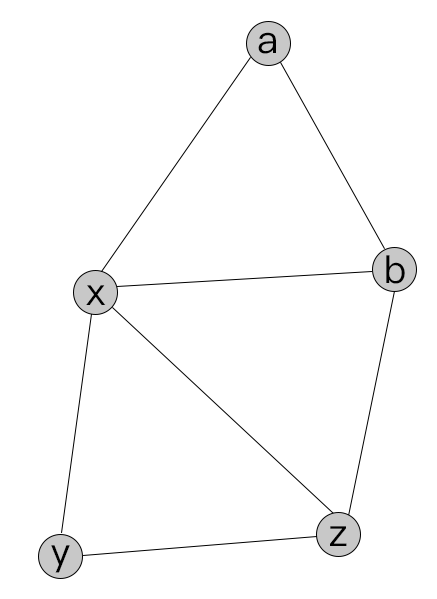
\includegraphics[width=0.2\textwidth]{3_figure.png}
        \caption{Example graph}
        \label{fig:ex}
    \end{figure}

    Given a formula $\phi$, we create a node for each literals and connect every pair of iterals in a clause. 
    For example, figure~\ref{fig:ex} is created according to the example formula given in this problem.



    This transformation can be done by iterating all clauses in a formula in polynomial time.
    Also, we notice that in order to make it possible to transform a graph to a \textsc{cnf} formula, we need to constrain that 
    \emph{every node in the graph must form at least one complete subgraph with two other nodes}. 

    \begin{theo}
        We can find solutions to $\sat$-1 if we have solutions to 3-\textsc{Coloring}.
    \end{theo}
    \begin{proof}
        Suppose a graph $G$ is given representing a \textsc{cnf} formula $\phi$ and we have a solution to the 3-\textsc{Coloring} 
        problem in $G$. We know that adjacent nodes cannot have the same color, so correspondingly, every literal in a clause 
        must be assigned a distinct color. Let's say a red node means that the corresponding literal is true, and the rest of the 
        literals are false. Since the graph must satisfy our constraint to be transformed to a \textsc{cnf} formula, 
        we know that for every three completely connected nodes(representing a clause), we have one and only one red node, meaning 
        that we have one and only one true literal in every clause, constructing a solution to $\sat$-1. The same works for the 
        other two colors. Thus, we prove that \underline{we can find solutions to $\sat$-1 if we have solutions to 3-\textsc{Coloring}}. 
        Setting the literals with one color to be true and others to be false is the solution to $\sat$-1.
    \end{proof}

    \begin{theo}
        We can find solutions for 3-\textsc{Coloring} if we have solutions for $\sat$-1.
    \end{theo}
    \begin{proof}
        To prove this, we are going to prove if there isn't a solution to $\sat$-1, there isn't a solution to 3-\textsc{Coloring} 
        either. Same as above, suppose we have $G$ and corresponding $\phi$. If there isn't a solution to $\sat$-1, which means 
        that we cannot find an arrangement of true and false for the literals to ensuring both $\phi$ to be true and there is only 
        one true literal in each clause. For example, consider equation~\ref{eqn:phi}, the corresponding graph $G'$ is shown in figure 
        \ref{fig:phi}. After playing around with $\phi'$, one should find that there is no way to make $\phi'$ true while ensuring 
        only one true literal is in each clause. To make $\phi'$ true, at least one clause would have two true literals. 
        This means if we are using three colors to fill $G'$, we cannot avoid filling two nodes with the same color at some point. 
        Thus we don't have a solution for the 3-\textsc{Coloring} problem. Therefore, we prove that \underline{if there isn't a solution to $\sat$-1, 
        there isn't a solution to 3-\textsc{Coloring} either}, which means the same thing as the theorem. 

        \begin{equation}
            \phi' = (x \vee y \vee z) \wedge (x \vee y \vee a) \wedge (a \vee y \vee z) \wedge (x \vee z \vee a)
            \label{eqn:phi}
        \end{equation}
        
        \begin{figure}
            \centering
            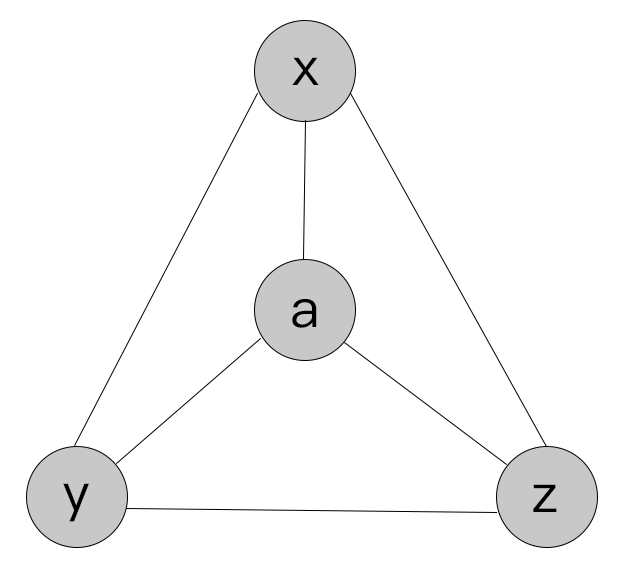
\includegraphics[width=0.2\textwidth]{3_phi.png}
            \caption{$G'$}
            \label{fig:G}
        \end{figure}
    \end{proof}

    Since 3-\textsc{Coloring} is $\NP$-complete, we prove that \underline{$\sat$-1 is $\NP$-complete}.
